\documentclass[fontset=windows]{article}
\usepackage{ctex}
\usepackage{lmodern}
\usepackage{tikz}
\usepackage{epigraph}
\usepackage{setspace}
\usepackage[a4paper,left=14mm,right=14mm,top=10mm,bottom=10mm]{geometry} 
\linespread{1.4}
\begin{document}
\section{9.14}
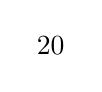
\begin{tikzpicture}[level distance=1.3cm,
        level 1/.style={sibling distance=3cm, level distance=1cm},
        level 2/.style={sibling distance=1.5cm, level distance=0.8cm}]
    \node {20};
\end{tikzpicture}

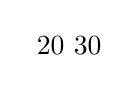
\begin{tikzpicture}[level distance=1.3cm,
        level 1/.style={sibling distance=3cm, level distance=1cm},
        level 2/.style={sibling distance=1.5cm, level distance=0.8cm}]
    \node {20 30};
\end{tikzpicture}

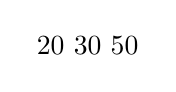
\begin{tikzpicture}[level distance=1.3cm,
        level 1/.style={sibling distance=3cm, level distance=1cm},
        level 2/.style={sibling distance=1.5cm, level distance=0.8cm}]
    \node {20 30 50};
\end{tikzpicture}

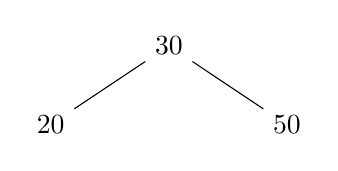
\begin{tikzpicture}[level distance=1.3cm,
        level 1/.style={sibling distance=3cm, level distance=1cm},
        level 2/.style={sibling distance=1.5cm, level distance=0.8cm}]
    \node {30}
    child {node{20}}
    child {node{50}};
\end{tikzpicture}

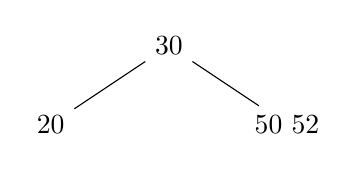
\begin{tikzpicture}[level distance=1.3cm,
        level 1/.style={sibling distance=3cm, level distance=1cm},
        level 2/.style={sibling distance=1.5cm, level distance=0.8cm}]
    \node {30}
    child {node{20}}
    child {node{50 52}};
\end{tikzpicture}

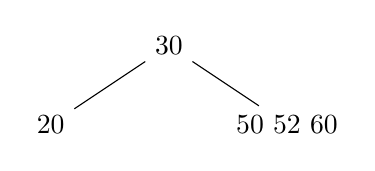
\begin{tikzpicture}[level distance=1.3cm,
        level 1/.style={sibling distance=3cm, level distance=1cm},
        level 2/.style={sibling distance=1.5cm, level distance=0.8cm}]
    \node {30}
    child {node{20}}
    child {node{50 52 60}};
\end{tikzpicture}

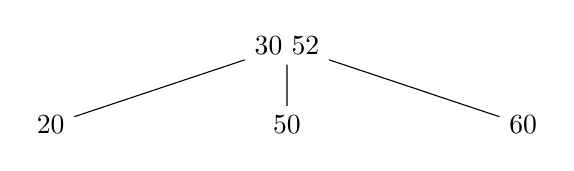
\begin{tikzpicture}[level distance=1.3cm,
        level 1/.style={sibling distance=3cm, level distance=1cm},
        level 2/.style={sibling distance=1.5cm, level distance=0.8cm}]
    \node {30 52}
    child {node{20}}
    child {node{50}}
    child {node{60}};
\end{tikzpicture}

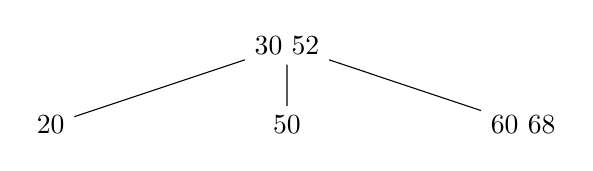
\begin{tikzpicture}[level distance=1.3cm,
        level 1/.style={sibling distance=3cm, level distance=1cm},
        level 2/.style={sibling distance=1.5cm, level distance=0.8cm}]
    \node {30 52}
    child {node{20}}
    child {node{50}}
    child {node{60 68}};
\end{tikzpicture}

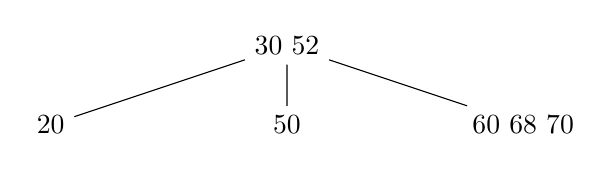
\begin{tikzpicture}[level distance=1.3cm,
        level 1/.style={sibling distance=3cm, level distance=1cm},
        level 2/.style={sibling distance=1.5cm, level distance=0.8cm}]
    \node {30 52}
    child {node{20}}
    child {node{50}}
    child {node{60 68 70}};
\end{tikzpicture}

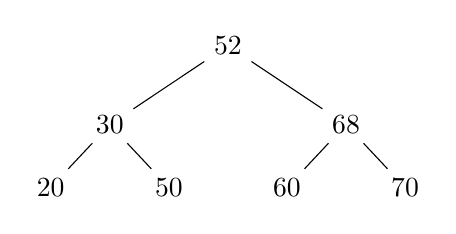
\begin{tikzpicture}[level distance=1.3cm,
        level 1/.style={sibling distance=3cm, level distance=1cm},
        level 2/.style={sibling distance=1.5cm, level distance=0.8cm}]
    \node {52}
    child {node{30}
            child{node{20}}
            child{node{50}}
        }
    child {node{68}
            child{node{60}}
            child{node{70}}
        };
\end{tikzpicture}
\\
\qquad 删除50:\\
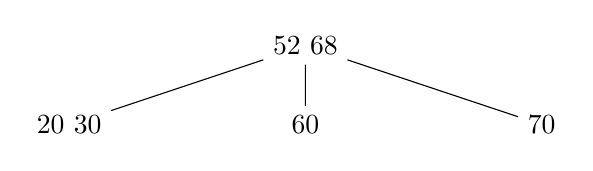
\begin{tikzpicture}[level distance=1.3cm,
        level 1/.style={sibling distance=3cm, level distance=1cm},
        level 2/.style={sibling distance=1.5cm, level distance=0.8cm}]
    \node {52 68}
    child{node{20 30}}
    child{node{60}}
    child{node{70}};
\end{tikzpicture}
\\
\qquad 删除68:\\
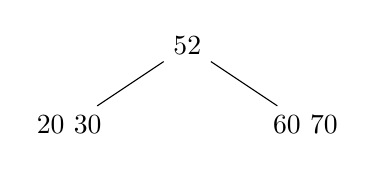
\begin{tikzpicture}[level distance=1.3cm,
        level 1/.style={sibling distance=3cm, level distance=1cm},
        level 2/.style={sibling distance=1.5cm, level distance=0.8cm}]
    \node {52}
    child {node{20 30}}
    child {node{60 70}};
\end{tikzpicture}

\section{9.15}
高度为$h$的三阶B-树,每一层最多节点:
$$k=1------------3^{0}$$
$$k=2------------3^{1}$$
$$k=3------------3^{2}$$
$$k=4------------3^{3}$$
\begin{center}
    \quad\vdots
\end{center}
$$k=h------------3^{h-1}$$
\qquad 高度为$h$的三阶B-树,每一层最少节点:
$$k=1------------\lceil\frac{3}{2}\rceil^{0}$$
$$k=2------------\lceil\frac{3}{2}\rceil^{1}$$
$$k=3------------\lceil\frac{3}{2}\rceil^{2}$$
$$k=4------------\lceil\frac{3}{2}\rceil^{3}$$
\begin{center}
    \quad\vdots
\end{center}
$$k=h------------\lceil\frac{3}{2}\rceil^{h-1}$$
\qquad 则叶子节点数目:\quad$[2^{h-1},3^{h-1}]$
\end{document}